\documentclass[12pt]{article}
%\usepackage{latexsym,amsmath,graphicx}
%\usepackage[top=2cm, bottom=2cm, left=2cm, right=2cm]{geometry}
\usepackage{fullpage,latexsym,amsmath,graphicx}
\setlength{\textheight}{25cm}
\pagestyle{empty}
\title{on random hex (draft)}
\author{RBH etc}
\date{April 2013}
\begin{document}
\maketitle
\section{intro}
Consider a game of random Hex on an $n$$\times$$n$ board.
Black and White alternate moves, and the first player to connect their two opposing sides wins. Each move is uniformly randomly selected
from the set of all available moves (i.e., empty cells) at that point.
For each player, and for each positive integer $t$,
we are interested in $w_n^t$, the probability that the player wins the game with their $t$'th move.

Hex on an $n$$\times$$n$ board has certain symmetries that simplify the computation of $w$.

Define $f_n^t$ as the probability that, 
a uniformly randomly chosen
$t$-subset of the $n$$\times$$n$ cell locations yields a winning configuration
for a fixed player --- say Black.
By the symmetry of the $n$$\times$$n$ board, and since 
each filled board yields a win for exactly one player (draws are not possible in Hex),
there is a bijection between $t$-subsets that
yield a win for Black and $t$-subsets that yield a win for White.
Thus $f_n^t$ is the same for each player.

Since each move is uniform random, 
$f_n^t$ is just the cumulative distribution of $w_n^t$,
namely
\[ f_n^t = \sum_{j=1}^t w_n^j \: .  \]


%% GNUPLOT: LaTeX picture with Postscript
\begingroup
  \makeatletter
  \providecommand\color[2][]{%
    \GenericError{(gnuplot) \space\space\space\@spaces}{%
      Package color not loaded in conjunction with
      terminal option `colourtext'%
    }{See the gnuplot documentation for explanation.%
    }{Either use 'blacktext' in gnuplot or load the package
      color.sty in LaTeX.}%
    \renewcommand\color[2][]{}%
  }%
  \providecommand\includegraphics[2][]{%
    \GenericError{(gnuplot) \space\space\space\@spaces}{%
      Package graphicx or graphics not loaded%
    }{See the gnuplot documentation for explanation.%
    }{The gnuplot epslatex terminal needs graphicx.sty or graphics.sty.}%
    \renewcommand\includegraphics[2][]{}%
  }%
  \providecommand\rotatebox[2]{#2}%
  \@ifundefined{ifGPcolor}{%
    \newif\ifGPcolor
    \GPcolorfalse
  }{}%
  \@ifundefined{ifGPblacktext}{%
    \newif\ifGPblacktext
    \GPblacktexttrue
  }{}%
  % define a \g@addto@macro without @ in the name:
  \let\gplgaddtomacro\g@addto@macro
  % define empty templates for all commands taking text:
  \gdef\gplbacktext{}%
  \gdef\gplfronttext{}%
  \makeatother
  \ifGPblacktext
    % no textcolor at all
    \def\colorrgb#1{}%
    \def\colorgray#1{}%
  \else
    % gray or color?
    \ifGPcolor
      \def\colorrgb#1{\color[rgb]{#1}}%
      \def\colorgray#1{\color[gray]{#1}}%
      \expandafter\def\csname LTw\endcsname{\color{white}}%
      \expandafter\def\csname LTb\endcsname{\color{black}}%
      \expandafter\def\csname LTa\endcsname{\color{black}}%
      \expandafter\def\csname LT0\endcsname{\color[rgb]{1,0,0}}%
      \expandafter\def\csname LT1\endcsname{\color[rgb]{0,1,0}}%
      \expandafter\def\csname LT2\endcsname{\color[rgb]{0,0,1}}%
      \expandafter\def\csname LT3\endcsname{\color[rgb]{1,0,1}}%
      \expandafter\def\csname LT4\endcsname{\color[rgb]{0,1,1}}%
      \expandafter\def\csname LT5\endcsname{\color[rgb]{1,1,0}}%
      \expandafter\def\csname LT6\endcsname{\color[rgb]{0,0,0}}%
      \expandafter\def\csname LT7\endcsname{\color[rgb]{1,0.3,0}}%
      \expandafter\def\csname LT8\endcsname{\color[rgb]{0.5,0.5,0.5}}%
    \else
      % gray
      \def\colorrgb#1{\color{black}}%
      \def\colorgray#1{\color[gray]{#1}}%
      \expandafter\def\csname LTw\endcsname{\color{white}}%
      \expandafter\def\csname LTb\endcsname{\color{black}}%
      \expandafter\def\csname LTa\endcsname{\color{black}}%
      \expandafter\def\csname LT0\endcsname{\color{black}}%
      \expandafter\def\csname LT1\endcsname{\color{black}}%
      \expandafter\def\csname LT2\endcsname{\color{black}}%
      \expandafter\def\csname LT3\endcsname{\color{black}}%
      \expandafter\def\csname LT4\endcsname{\color{black}}%
      \expandafter\def\csname LT5\endcsname{\color{black}}%
      \expandafter\def\csname LT6\endcsname{\color{black}}%
      \expandafter\def\csname LT7\endcsname{\color{black}}%
      \expandafter\def\csname LT8\endcsname{\color{black}}%
    \fi
  \fi
  \setlength{\unitlength}{0.0500bp}%
  \begin{picture}(7200.00,5040.00)%
    \gplgaddtomacro\gplbacktext{%
      \csname LTb\endcsname%
      \put(1078,704){\makebox(0,0)[r]{\strut{} 0}}%
      \put(1078,1439){\makebox(0,0)[r]{\strut{} 0.02}}%
      \put(1078,2174){\makebox(0,0)[r]{\strut{} 0.04}}%
      \put(1078,2909){\makebox(0,0)[r]{\strut{} 0.06}}%
      \put(1078,3644){\makebox(0,0)[r]{\strut{} 0.08}}%
      \put(1078,4379){\makebox(0,0)[r]{\strut{} 0.1}}%
      \put(1758,484){\makebox(0,0){\strut{} 20}}%
      \put(2855,484){\makebox(0,0){\strut{} 40}}%
      \put(3952,484){\makebox(0,0){\strut{} 60}}%
      \put(5048,484){\makebox(0,0){\strut{} 80}}%
      \put(6145,484){\makebox(0,0){\strut{} 100}}%
      \put(176,2541){\rotatebox{-270}{\makebox(0,0){\strut{}win rate on that move}}}%
      \put(4006,154){\makebox(0,0){\strut{}move number}}%
      \put(4006,4709){\makebox(0,0){\strut{}Hex win rates by move}}%
    }%
    \gplgaddtomacro\gplfronttext{%
      \csname LTb\endcsname%
      \put(1606,4206){\makebox(0,0)[r]{\strut{}??}}%
    }%
    \gplbacktext
    \put(0,0){\includegraphics{code/data/gn/winrate.11.eps}}%
    \gplfronttext
  \end{picture}%
\endgroup

\ \hfill 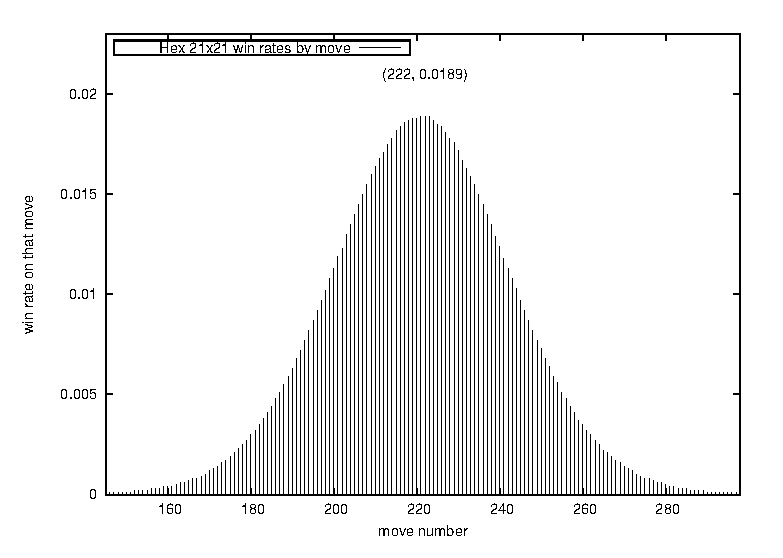
\includegraphics{code/data/gn/winrate.21.eps} \hfill \ 

\ \hfill 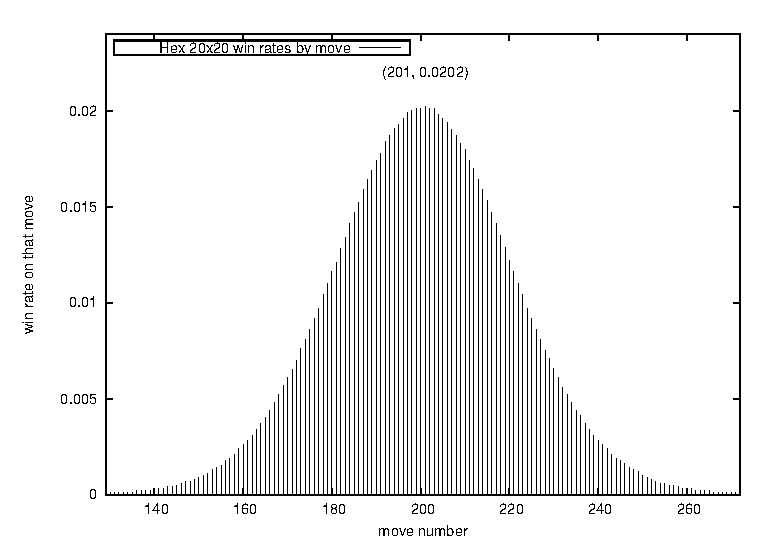
\includegraphics{code/data/gn/winrate.20.eps} \hfill \ 

\ \hfill 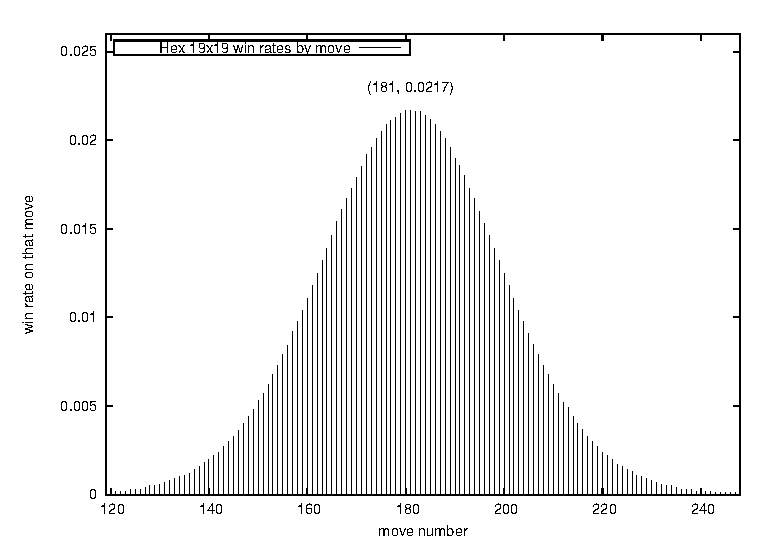
\includegraphics{code/data/gn/winrate.19.eps} \hfill \ 

\ \hfill \includegraphics{code/data/gn/winrate.18.eps} \hfill \ 

\ \hfill \includegraphics{code/data/gn/winrate.17.eps} \hfill \ 

\ \hfill \includegraphics{code/data/gn/winrate.16.eps} \hfill \ 

\ \hfill \includegraphics{code/data/gn/winrate.15.eps} \hfill \ 

\ \hfill 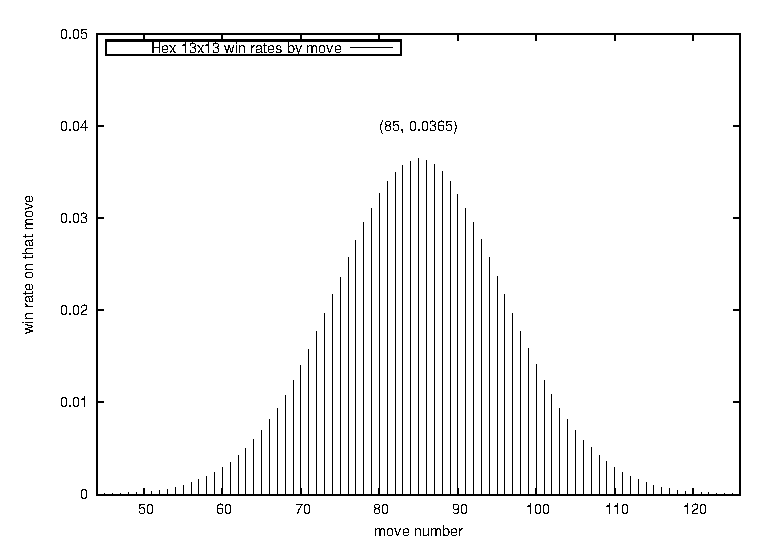
\includegraphics{code/data/gn/winrate.13.eps} \hfill \ 

\ \hfill \includegraphics{code/data/gn/winrate11.eps} \hfill \ 

\ \hfill \includegraphics{code/data/gn/winrate.9.eps} \hfill \ 

\ \hfill \includegraphics{code/data/gn/winrate.7.eps} \hfill \ 

\ \hfill \includegraphics{code/data/gn/winrate.5.eps} \hfill \ 

\ \hfill \includegraphics{code/data/gn/winrate.3.eps} \hfill \ 

\section{random hex win prob \ \ (draft ??)}
define $b(n)$ (resp.\ $w(n)$)
as probability that first (second) player wins $n$$\times$$n$ hex

Once one player has a connection, filling any unoccupied cells
does not change the outcome.
So $b(n)$ is the fraction
of final board positions (exactly $\lceil n^2/2 \rceil$ black cells)
that connect black's two sides, 
$w(n)$ is the fraction
of final board positions (exactly $\lfloor n^2/2 \rfloor$ white cells)
that connect white's two sides.
Flipping colors and reflecting through the main
diagonal maps a winning position to a winning position,
and so $b(n)=w(n)$ if $n$ is even.

\section{n odd}
For $n=2t+1$, we are interested in $b(n)-w(n)$.
Any corresponding position corresponds 
to a game that black wins on the last move;
after the initial $n-1$ stones have been played, the
black subset is not winning, and neither is the white.
The white subset is a non-winning $t$-subset,
the black subset is a non-winning $t$-subset,
which the final stone transforms into a winning $t+1$-subset.
Thus the last stone is a cut vertex of the final winning
black connecting set.
So this difference can be found by finding the 
ratio $c(n)$ of cut vertices to total vertices over
all black winning subsets.
\[ c(n) = \frac{b(n)-w(n)}{b(n)} 
\: \: \: \: \: \mbox{\rm and } \: \: \: \: \:  
b(n) + w(n) = 1
\: \: \: \: \: \mbox{\rm so }  \: \: \: \: \: 
b(n) = \frac{1}{2 - c(n)}\] 
so $b(n)$ goes to 0.5 if $c(n)$ goes to 0.

\vfill

\noindent{\bf Data generated by counting subsets}

\begin{tabular}{ccccccc}
$n$ & subsets & w-win & b-win & $w(n)$ & $b(n)$ & $c(n)$ \\
1   &  1      &  0    & 1     & 1         & 0     &  1     \\
3   &  126    & 42    & 84    & .333333... & .666666... & .5 \\
5   &  5200300 &  2219059 & 2981241 & .426717... & .573282... & .255659... 
\end{tabular}

\vfill

\noindent{\bf Data generated by $10^6$ pseudorandom samples, error about .001}

\begin{verbatim}
 3 .332755 .667051
 5 .427192 .573638
 7 .456181 .544021
 9 .469588 .530459
11 .476214 .522408
13 .482711 .519231
15 .485096 .515169
17 .487105 .512194
19 .489548 .511278
21 .491369 .510176
23 .491933 .508733
25 .492264 .507082
\end{verbatim}
\newpage
\vspace*{-3cm}
{\small\bf
\begin{verbatim}
 . . .    . . .    . . .    . . .    . . .    . . .    . . .    . . .    . . .   
  . . 1    . 1 .    . 1 1    . 1 1    . 1 1    1 . .    1 . 1    1 . 1    1 . 1   
   1 1 1    1 1 1    . 1 1    1 . 1    1 1 .    1 1 1    . 1 1    1 . 1    1 1 .   

 . . .    . . .    . . .    . . .    . . .    . . .    . . 1    . . 1    . . 1   
  1 1 .    1 1 .    1 1 .    1 1 1    1 1 1    1 1 1    . . .    . . 1    . . 1   
   . 1 1    1 . 1    1 1 .    . . 1    . 1 .    1 . .    1 1 1    . 1 1    1 . 1   

 . . 1    . . 1    . . 1    . . 1    . . 1    . . 1    . . 1    . . 1    . . 1   
  . . 1    . 1 .    . 1 .    . 1 .    . 1 1    . 1 1    . 1 1    1 . .    1 . .   
   1 1 .    . 1 1    1 . 1    1 1 .    . . 1    . 1 .    1 . .    . 1 1    1 . 1   

 . . 1    . . 1    . . 1    . . 1    . . 1    . . 1    . . 1    . . 1    . 1 .   
  1 . .    1 . 1    1 . 1    1 . 1    1 1 .    1 1 .    1 1 .    1 1 1    . . .   
   1 1 .    . . 1    . 1 .    1 . .    . . 1    . 1 .    1 . .    . . .    1 1 1   

 . 1 .    . 1 .    . 1 .    . 1 .    . 1 .    . 1 .    . 1 .    . 1 .    . 1 .   
  . . 1    . . 1    . . 1    . 1 .    . 1 .    . 1 .    . 1 1    . 1 1    . 1 1   
   . 1 1    1 . 1    1 1 .    . 1 1    1 . 1    1 1 .    . . 1    . 1 .    1 . .   

 . 1 .    . 1 .    . 1 .    . 1 .    . 1 .    . 1 .    . 1 .    . 1 .    . 1 .   
  1 . .    1 . .    1 . .    1 . 1    1 . 1    1 . 1    1 1 .    1 1 .    1 1 .   
   . 1 1    1 . 1    1 1 .    . . 1    . 1 .    1 . .    . . 1    . 1 .    1 . .   

 . 1 .    . 1 1    . 1 1    . 1 1    . 1 1    . 1 1    . 1 1    . 1 1    . 1 1   
  1 1 1    . . .    . . .    . . .    . . 1    . . 1    . . 1    . 1 .    . 1 .   
   . . .    . 1 1    1 . 1    1 1 .    . . 1    . 1 .    1 . .    . . 1    . 1 .   

 . 1 1    . 1 1    . 1 1    . 1 1    . 1 1    . 1 1    . 1 1    1 . .    1 . .   
  . 1 .    . 1 1    1 . .    1 . .    1 . .    1 . 1    1 1 .    . . .    . . 1   
   1 . .    . . .    . . 1    . 1 .    1 . .    . . .    . . .    1 1 1    . 1 1   

 1 . .    1 . .    1 . .    1 . .    1 . .    1 . .    1 . .    1 . .    1 . .   
  . . 1    . . 1    . 1 .    . 1 .    . 1 .    . 1 1    . 1 1    . 1 1    1 . .   
   1 . 1    1 1 .    . 1 1    1 . 1    1 1 .    . . 1    . 1 .    1 . .    . 1 1   

 1 . .    1 . .    1 . .    1 . .    1 . .    1 . .    1 . .    1 . .    1 . .   
  1 . .    1 . .    1 . 1    1 . 1    1 . 1    1 1 .    1 1 .    1 1 .    1 1 1   
   1 . 1    1 1 .    . . 1    . 1 .    1 . .    . . 1    . 1 .    1 . .    . . .   

 1 . 1    1 . 1    1 . 1    1 . 1    1 . 1    1 . 1    1 . 1    1 . 1    1 . 1   
  . . .    . . .    . . .    . . 1    . . 1    . . 1    . 1 .    . 1 .    . 1 .   
   . 1 1    1 . 1    1 1 .    . . 1    . 1 .    1 . .    . . 1    . 1 .    1 . .   

 1 . 1    1 . 1    1 . 1    1 . 1    1 . 1    1 . 1    1 1 .    1 1 .    1 1 .   
  . 1 1    1 . .    1 . .    1 . .    1 . 1    1 1 .    . . .    . . .    . . .   
   . . .    . . 1    . 1 .    1 . .    . . .    . . .    . 1 1    1 . 1    1 1 .   

 1 1 .    1 1 .    1 1 .    1 1 .    1 1 .    1 1 .    1 1 .    1 1 .    1 1 .   
  . . 1    . . 1    . . 1    . 1 .    . 1 .    . 1 .    . 1 1    1 . .    1 . .   
   . . 1    . 1 .    1 . .    . . 1    . 1 .    1 . .    . . .    . . 1    . 1 .   

 1 1 .    1 1 .    1 1 .    1 1 1    1 1 1    1 1 1    1 1 1    1 1 1    1 1 1   
  1 . .    1 . 1    1 1 .    . . .    . . .    . . .    . . 1    . 1 .    1 . .   
   1 . .    . . .    . . .    . . 1    . 1 .    1 . .    . . .    . . .    . . .   
\end{verbatim}

\newpage
\section{probs}
using sampling, we approximate the prob that a particular
cell is the black winning move (namely, that the game ends with that move)

eg. on 3x3, prob a1 wins?
\begin{verbatim}
winning path
! . .        
 x . .
  x . .
wins on move 3 prob (1/(9 choose 2)) * 1/7
wins on move 4 prob (5/(9 choose 3)) * 1/6
wins on move 5 prob (9/(9 choose 4)) * 1/5
! . .        (not the above => bottom left cell not black)
 x x .
  . x .
wins on move 4 prob (1/(9 choose 3)) * 1/6
wins on move 5 prob (2/(9 choose 4)) * 1/5
! . .        
 x x x
  . . x
wins on move 5 prob (1/(9 choose 4)) * 1/5

total
(1/(9 choose 2))*1/7 + (1/(9 choose 3)) + (12/5)(1/(9 choose 4)) = 
11/(9*7*5) = 0.0349206349...

by contrast, the prob that black wins after playing at a1
is 12/126 = 0.095238...
\end{verbatim}

prob game goes to last move is 1 - 2*prob(n2-1)/2 stones connect
= prob (n2-1)/2 stones connect in neither direction

\newpage
\ \hfill 
\includegraphics[scale=1]{draw/bigboard.eps} \hfill \ 



\end{document}
